\def\mytitle{IMPLEMENTATION OF RANDOM GENERATOR USING\\ D FLIPFLOPS IN ARDUINO IDE}
\def\mykeywords{}
\def\myauthor{MARIKUNDAM HARSHITHA}
\def\contact{marikundamdec@gmail.com}
\def\mymodule{}
\documentclass[10pt,a4paper]{article}
\usepackage[a4paper,outer=1.5cm,inner=1.5cm,top=1.75    cm,bottom=1.5cm]{geometry}
%  \twocolumn
\usepackage{graphicx}
\usepackage{amsfonts}
\usepackage{circuitikz}
\usetikzlibrary{calc}
\usepackage{subcaption}
\usepackage{tikz}
\usepackage{amsmath}
\usepackage[margin=1cm]{geometry}
%\usetikzlibrary{shapes.geometric}
\usetikzlibrary{shapes,arrows,chains,decorations.markings,intersections,calc}
\usepackage{lipsum}
\usetikzlibrary{positioning}
\usepackage{xcolor}
\usepackage{multirow}
\usepackage{listings}
\usepackage{float}
\usepackage{titlesec}
\usepackage{amsmath}
\usepackage[utf8]{inputenc}
\usepackage{tabularx}
\usepackage{algorithm2e}
\usepackage{./karnaugh-map}
\usepackage{capt-of}
\usepackage{caption}                             
\usepackage{datetime}
\usepackage{lipsum}
\usepackage{amsmath}
\usepackage{textgreek}
\usepackage{tabularx}
\usepackage{circuitikz}
\usepackage{tikz}
\usetikzlibrary{calc}                         
\usetikzlibrary{circuits.logic.US}
\title{\mytitle}
 \author{\myauthor\hspace{1em}\\\contact\\FWC22120        IITH-Future Wireless Communications     Assignment    -1\hspace{0.5em}\hspace{0.5em}\mymodule}
\date{}
\sloppy
\lstset{                                          
language=C++,                           
basicstyle=\ttfamily\footnotesize,   
breaklines=true,                       
frame=lines
}

\begin{document}
\maketitle
\tableofcontents

\section{Problem}
(GATE2021-QP-EC)\\
Q.46 The propogation delay of he exclusve-OR(XOR) gate in the circuit in the figure is 3ns.The ropogation delay of all the flip-flops is assumned to be zero.The clock(Clk) frequency provided to the circuit is 500MHz.\\
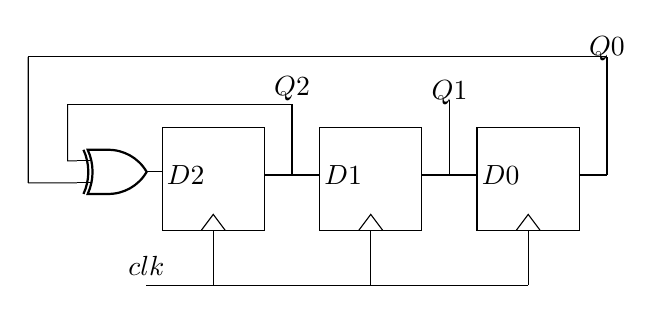
\begin{tikzpicture}
\ctikzset{                                   
logic ports=ieee,                   
logic ports/scale=0.5               
}                                    
\draw(-1.3,-0.56)node[xor port,anchor=out](x) {};  
%Drawing flip-flops
\draw (-1.3,-1.3) rectangle (0,0);
\draw(-1,-0.6) node{$D2$};
\draw(0.7,-1.3) rectangle (2,0);
\draw(1,-0.6) node{$D1$};
\draw(2.7,-1.3) rectangle (4,0);
\draw(3,-0.6) node{$D0$};
%connecting them
\draw(0,-0.6) -- (0.7,-0.6);
\draw(2,-0.6) -- (2.7,-0.6);
\draw(4,-0.6) -- (4.35,-0.6);
%drawing clk
\draw(-1.5,-2) node[above]{$clk$} -- (3.35,-2);
%connecting clk 
\draw(-0.65,-2) -- (-0.65,-1.3);
\draw(1.35,-2) -- (1.35,-1.3);
\draw(3.35,-2) -- (3.35,-1.3);
%drawing clk edges
\draw(-0.5,-1.3) -- (-0.65,-1.1) -- (-0.8,-1.3);
\draw(1.2,-1.3) -- (1.35,-1.1) -- (1.5,-1.3);
\draw(3.2,-1.3) -- (3.35,-1.1) -- (3.5,-1.3);
%drawing Q2,Q1,Q0
\draw(0.35,-0.6) --(0.35,0.3);
\draw(2.35,-0.6) --(2.35,0.35);
\draw(4.35,-0.6) --(4.35,0.9);
\draw(4.35,0.9) -- (-3,0.9);
\draw(0.35,0.3) -- (-2.5,0.3);
\draw(x.in 2) -|(-3,-0.7)to[short](-3,0.9);
\draw(x.in 1) -|(-2.5,-0.3)to[short](-2.5,0.3);
\draw(0.35,0.5)node{$Q2$};
\draw(2.35,0.45)node{$Q1$};
\draw(4.35,1)node{$Q0$};
\end{tikzpicture}

Starting from the initial value of the flip-flop outputs $Q2Q1Q0 =111$ with $D2=1$,the minimum number of triggering clock edges after which the flip-flop outputs $Q2Q1Q0$ becomes 1 0 0\emph{(in integer)} is \line(1,0){10}

\section{Introduction}
A random numbe generator using D flip-flops is a simple digital circuit that generates a sequence of random binary numbers.To implement this type of random number generator, we use a series of D flip-flops connected in a feedback loop. The output of each flip-flop is fed back into the input of the next flip-flop,creating a circuit that generated a sequence of random binary values.\\ \\
The feedback loop creates a delay in the circuit,which causes the circuit to exhibit unpredictable behavior.This unpredictable behavior results in a sequence of random binary values. The length of the delay can be adjusted to control the randomness of the output.

\section{Components}


\begin{tabular}{|p{3cm}|p{3cm}|p{3cm}|}
\hline                                        
\textbf{Symbol} & \textbf{Values} & \textbf{Description}\\                                          
\hline                                 
$\theta$ & 30$\degree{}$   & $\angle{BAD} = \angle{BAC}$ \\           
\hline                                    
a &  9 & $AB$ \\     
\hline                      
c & 5 & $AC$ \\
\hline                                     
		$\vec{e}_1$ & $\myvec{
			1\\
			0\\
			}$ & basis vector\\ 
\hline
\end{tabular}


\subsection{Arduino} \vspace{5mm}
The Arduino Uno has some ground pins,analog input pins A0-A3 and digital pins D1-D13 that can be used for both input as well as output.It also has two power pins that can generate 3.3V and 5V.Inthe following exercises, we use digital pins,GND and 5V .
\subsection{Seven Segment Display} \vspace{5mm}
The seven segment display has eight pins, \emph{a,b,c,d,e,f,g} and \emph{dot} that take an active LOW input,i.e. the LED will glow only if the input is connected to ground.Each of these pins is connected to an LED segment.The \emph{dot} pin is reserved for the LED.
\section{Implementation}
A 7474IC which  has 14 pins and can store two seperate binary values.So we consider two IC's since we have three values  and connect the  D inputs of each flip-flop to the input signals of 7447IC . Later interface 7447IC to seven segment display for the output. The CLK input is used to trigger the flip-flop,and the Q output is used to read the stored value.When a positive edge is detected on the CLK input,the current value on the D input is stored in the flip-flop. The boolean expression of the D flip-flop is $Q(t+1) = D$
\subsection{Truth table}
\begin{tabular}{|p{2cm}|p{2cm}|p{2cm}|}
\hline
\multicolumn{3}{|c|}{Truth table}\\
\hline
R& S& A\\
\hline
0& 0& 0\\
\hline
0& 1& 1\\
\hline
1& 0& 1\\
\hline
1& 1& 0\\
\hline
\end{tabular}

\subsection{K-map}
Since $Q'= D$,we find the k-maps for D as outputs
\newline
\begin{figure}
\begin{karnaugh-map}[4][2][1][$Q2$ $Q1$][$Q0$]    
\minterms{2,3,4,5}                    
\maxterms{0,1,6,7}                
\implicant{3}{2}              
\implicant{4}{5}          
\end{karnaugh-map}
\caption{For $D2$}
\label{For $D2$}
\end{figure}


\begin{figure}
\begin{karnaugh-map}[4][2][1][$Q2$ $Q1$][$Q0$]  
\minterms{2,3,7,6}            
\maxterms{0,1,4,5}         
\implicant{3}{6}              
\end{karnaugh-map}
\caption{For $D1$}
	\label{For $D2$}
\end{figure}
   

\begin{figure}
\begin{karnaugh-map}[4][2][1][$Q2$ $Q1$][$Q0$]    
\minterms{1,3,5,7}                   
\maxterms{0,2,4,6}            
\implicant{1}{7}            
\end{karnaugh-map}
\caption{For $D0$}
	\label{For $D2$}
\end{figure}

\subsection{Boolean Equation}
By solving the K-maps above we obtain as follows :
\begin{align}
	D2 &= \overline{Q2}Q0 + \overline{Q0}Q2 \\
	D1 &= Q2 \\
	D0 &= Q1 
\end{align}
\section{Hardware}
\begin{enumerate}
\item Make the connections between the seven segment display and the 7447 IC as shown in Table3
\newline\newline
\begin{tabular}{|p{2cm}|p{1cm}|p{1cm}|p{1cm}|p{1cm}|p{1cm}|p{1cm}|p{1cm}|}        
\hline                                        
\textbf{7447} & $\overline{a}$ & $\overline{b}$ & $\overline{c}$ & $\overline{d}$ & $\overline{e}$ & $\overline{f}$ & $\overline{g}$ \\          
\hline                                             
\textbf{Display} & a & b & c & d & e & f & g \\
\hline
\end{tabular}

\item Connect the Arduino,7447 and the two 7474 ICs according to Table4
\newline\newline
\captionof{table}{Table4}
\label{table:4}
\begin{tabular}{|c|c|c|c|c|c|c|c|c|c|c|c|c|}      
\hline                              
\multirow{2}{*}{} & \multicolumn{3}{|c|}{INPUT} & \multicolumn{3}{|c|}{OUTPUT} & \multicolumn{2}    {|c|}{\multirow{2}{*}{CLOCK}} & \multicolumn{4}{|c|}    {\multirow{3}{*}{5V}} \\      
\cline{2-7}     
& Q0 & Q1 & Q2 & Q0' & Q1' & Q2' & \multicolumn{2}{|c|}{\multirow{2}{*}{}} & \multicolumn{4}{|c|}{} \\        
\hline          
Arduino & D6 & D7 & D8 & D2 & D3 & D4 & \multicolumn{2}{|c|}{D13} & \multicolumn{4}{|c|}{\multirow{3}{*}{}}\\                                   
\hline                             
7474 & 5 & 9 &  & 2 & 12 &  & CLK1 & CLK2 & 1 & 4 & 10 & 13 \\                   
\hline                     
7474 & & & 5 & & & 2 & CLK1 & CLK2 & 1 & 4  & 10 & 13 \\                       
\hline                         
7447 & \multicolumn{3}{|c|}{} & 7 & 1 & 2 & & & \multicolumn{4}{|c|}{16} \\              
\hline                     
\end{tabular}\\

\item Make the othet connections grounded , supply the 
5V and GND from the arduino as well.\\
\item When the clock edge is trigerred we observe display of random numbers.
\end{enumerate}
\section{Software}
Now write the following code and upload in arduino to see the results.
\newline\newline
\lstinputlisting{code6.cpp}
\end{document}
